A música esteve presente com a humanidade por séculos. Há diversas interpretações e a ela é atribuída diversos significados e intenções. Trata-se de uma manifestação artística e, assim como toda outra, há uma transmissão de informação entre criador, no caso, o compositor; e o consumidor, no caso, o ouvinte.

Além de transmitir informação, as composições musicais apresentem em alto nível, muitas vezes, ordem e padrões beme definidos. Podemos citar características como: estrutura, refrões, repetições, \textit{riffs}, etc.

Informação pode ser mensurada, e diversos estudos tem sido feitos na área há decadas, tendo Claude Shannon, o \"pai da teoria da informação\", desenvolvido um papel muito importante. \cite{shannon}

Com a notação musical utilizada há muitos anos, tem-se uma representação da música bem estruturada e discretizada. Há eventos bem definidos, durações, técnicas, etc. Este trabalho utiliza os conceitos estudados por Shannon e outros para tentar medir a quantidade de informação que uma música transmite.




    % \begin{figure}[ht]
    % \centering
    % 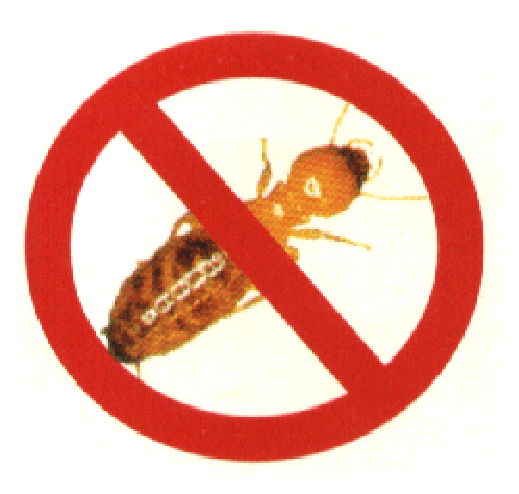
\includegraphics[width=0.5\textwidth]{Cap1/cupim}
    % \caption{Proibido estacionar cupins. Legenda grande, com o objetivo de demonstrar a indentação na lista de figuras.}
    % \label{cupim}
    % \end{figure}

    
    % \begin{figure}[ht!]
    % \centering
    % 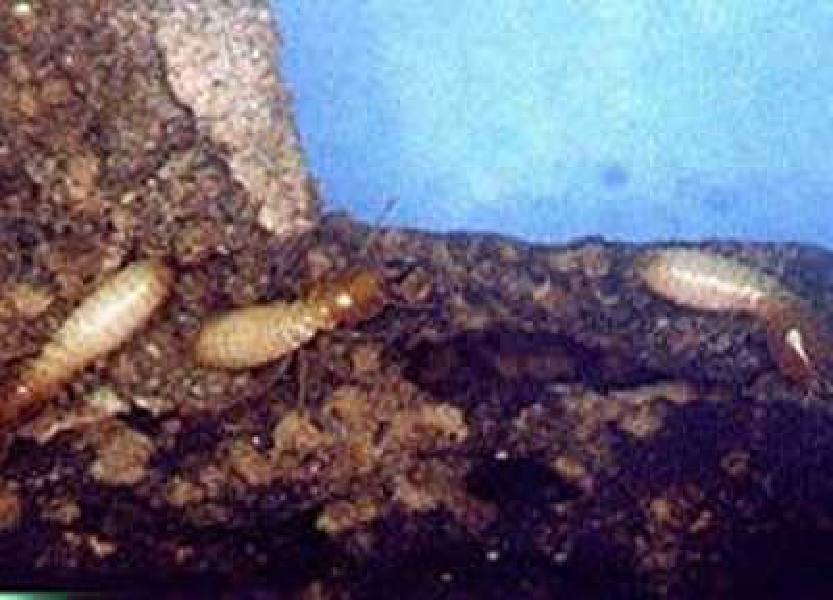
\includegraphics[width=1\textwidth]{Cap1/cupimconcreto}
    % \caption{Exemplo real de cupim frente ao seu dilema.}
    % \label{FDII}
    % \end{figure}
    
    % \begin{figure}[ht]
    % \centering
    % 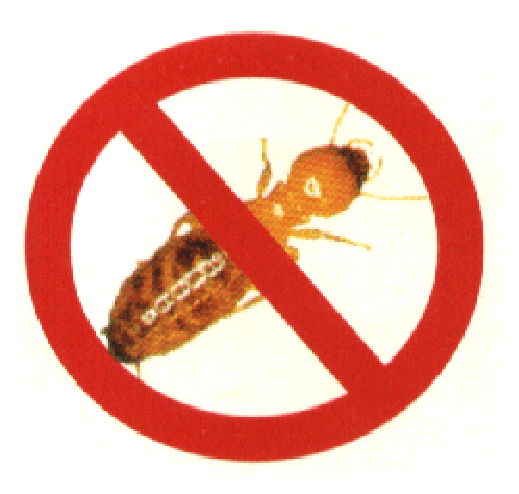
\includegraphics[width=0.5\textwidth]{Cap1/cupim}
    % \caption{Proibido estacionar cupins. Legenda grande, com o objetivo de demonstrar a indentação na lista de figuras.}
    % \label{cupim}
    % \end{figure}
    
    % \begin{figure}[ht!]
    % \centering
    % 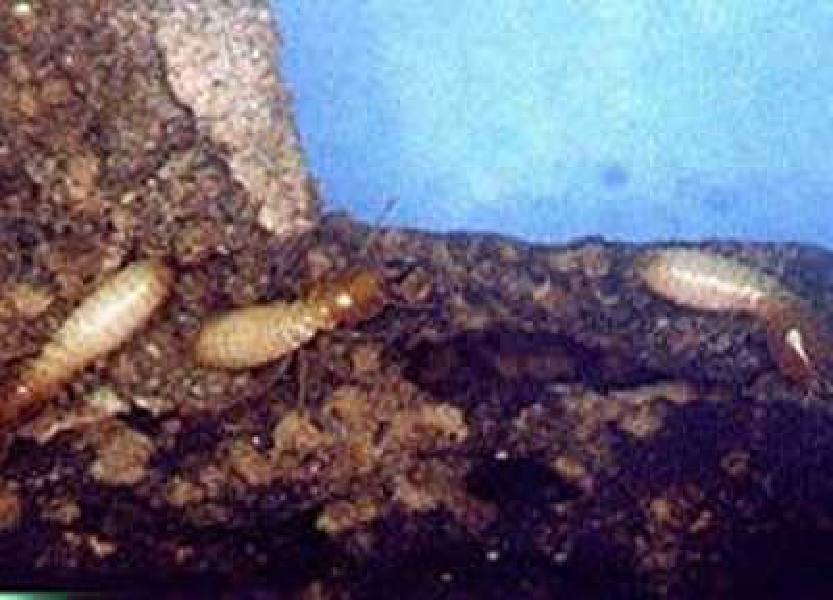
\includegraphics[width=1\textwidth]{Cap1/cupimconcreto}
    % \caption{Exemplo real de cupim frente ao seu dilema.}
    % \label{FDII}
    % \end{figure}
    